\chapter{Gruppenfilter}\label{gruppenfilter}
\minitoc
\clearpage
\section{Gruppenfilter}
Innerhalb von Excercises bzw. Übungen erscheint dieser Reiter/Tab, der es ermöglicht Abgaben nach Gruppen zu filtern. 

\begin{figure}
	\centering
	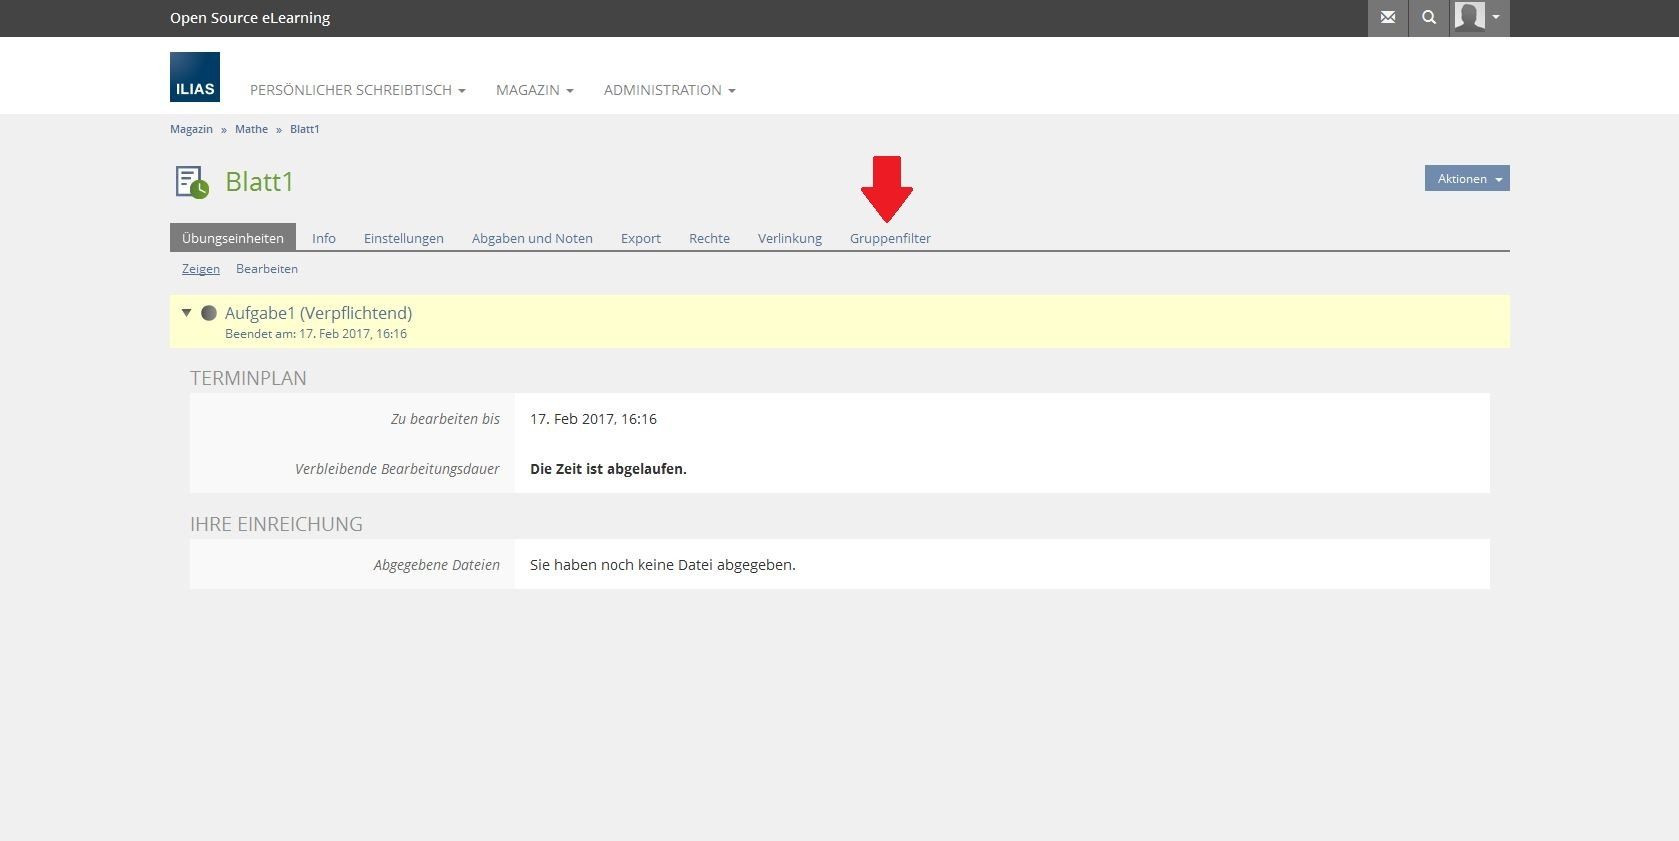
\includegraphics[width=1\textwidth]{img/excerciseGruppenfilter.jpg}
	\caption{Ansicht Gruppenfilter Tab}
\end{figure}

\subsection*{Unterpunkt}
\begin{itemize}
	\item Text Unterpunkt
\end{itemize}

\clearpage